\documentclass[a4paper,11pt]{article}
\usepackage[utf8]{inputenc}\usepackage[T1]{fontenc}
\usepackage[english]{babel}\usepackage{lmodern}\usepackage{microtype}
\usepackage{amsmath,amssymb}\usepackage{geometry}
\geometry{a4paper,left=2.2cm,right=2.2cm,top=2.0cm,bottom=2.0cm}
\usepackage{booktabs,array}\usepackage{xcolor}
\definecolor{bokug}{RGB}{0,135,60}\usepackage{tikz}
\usetikzlibrary{arrows.meta,calc}
\usepackage{fancyhdr}\pagestyle{fancy}
\renewcommand{\headrulewidth}{0.4pt}
\usepackage{enumitem}\setlength{\parindent}{0pt}\setlength{\parskip}{4pt}

\begin{document}
\fancyhead[L]{\small VU Mechanik – LAWI 100515 (PI)}\fancyhead[R]{\small SS 2026}\fancyfoot[C]{\thepage}
\begin{center}{\large\bfseries\color{bokug}University of Natural Resources and Life Sciences, Vienna (BOKU)}\\[2pt]{\large\bfseries VU Mechanik – LAWI 100515 (PI)}\\[4pt]Exam \textbf{Group A} \hfill Date: 26.06.2026\\[2pt]\rule{\linewidth}{0.4pt}\end{center}

\begin{center}\textbf{\large Model solution}\end{center}
\begin{center}
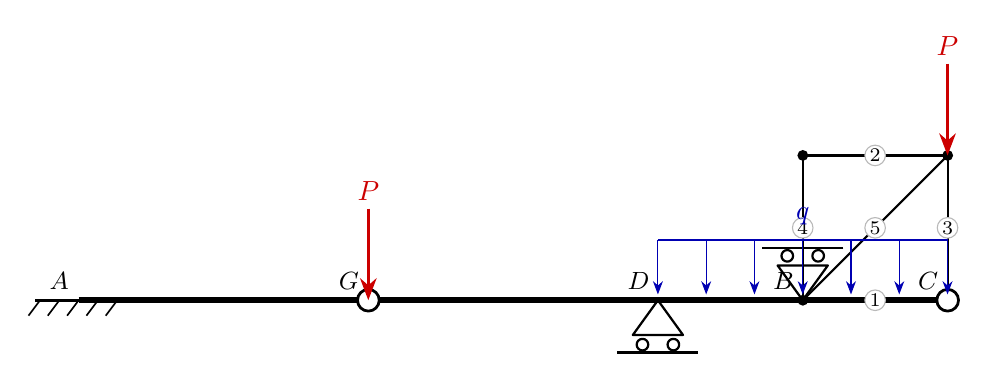
\begin{tikzpicture}[scale=1.226,>=Stealth,line join=round]
  \coordinate (P0) at (0.000,0.000);
  \coordinate (G) at (3.000,0.000);
  \coordinate (D) at (6.000,0.000);
  \coordinate (P1) at (9.000,0.000);
  \coordinate (TO1) at (7.500,0.000);
  \coordinate (TU0) at (9.000,1.500);
  \coordinate (TU1) at (7.500,1.500);
  \draw[thick] (P1) -- (TO1);
  \draw[thick] (TU0) -- (TU1);
  \draw[thick] (P1) -- (TU0);
  \draw[thick] (TO1) -- (TU1);
  \draw[thick] (TU0) -- (TO1);
  \draw[line width=2.2pt] (P0) -- (G);
  \draw[line width=2.2pt] (G) -- (D);
  \draw[line width=2.2pt] (D) -- (P1);
  \fill (P1) circle (1.6pt);
  \fill (TO1) circle (1.6pt);
  \fill (TU0) circle (1.6pt);
  \fill (TU1) circle (1.6pt);
  \draw[fill=white,line width=1pt] (P1) circle (3.2pt);
  \draw[fill=white,line width=1pt] (G) circle (3.2pt);
  \draw[line width=1.1pt] (-0.450,0.000) -- (0.450,0.000);
  \draw[line width=0.6pt] (-0.400,0.000) -- (-0.520,-0.160);
  \draw[line width=0.6pt] (-0.200,0.000) -- (-0.320,-0.160);
  \draw[line width=0.6pt] (0.000,0.000) -- (-0.120,-0.160);
  \draw[line width=0.6pt] (0.200,0.000) -- (0.080,-0.160);
  \draw[line width=0.6pt] (0.400,0.000) -- (0.280,-0.160);
  \draw[thick] (6.000,0.000) -- (5.740,-0.360) -- (6.260,-0.360) -- cycle;
  \draw[thick] (5.840,-0.460) circle (0.06) (6.160,-0.460) circle (0.06);
  \draw[line width=1pt] (5.580,-0.540) -- (6.420,-0.540);
  \draw[thick] (7.500,0.000) -- (7.760,0.360) -- (7.240,0.360) -- cycle;
  \draw[thick] (7.660,0.460) circle (0.06) (7.340,0.460) circle (0.06);
  \draw[line width=1pt] (7.920,0.540) -- (7.080,0.540);
  \node[circle,fill=white,draw=gray!55,inner sep=0.5pt,font=\scriptsize] at (8.250,0.000) {1};
  \node[circle,fill=white,draw=gray!55,inner sep=0.5pt,font=\scriptsize] at (8.250,1.500) {2};
  \node[circle,fill=white,draw=gray!55,inner sep=0.5pt,font=\scriptsize] at (9.000,0.750) {3};
  \node[circle,fill=white,draw=gray!55,inner sep=0.5pt,font=\scriptsize] at (7.500,0.750) {4};
  \node[circle,fill=white,draw=gray!55,inner sep=0.5pt,font=\scriptsize] at (8.250,0.750) {5};
  \draw[->,blue!70!black] (6.000,0.620) -- (6.000,0.060);
  \draw[->,blue!70!black] (6.500,0.620) -- (6.500,0.060);
  \draw[->,blue!70!black] (7.000,0.620) -- (7.000,0.060);
  \draw[->,blue!70!black] (7.500,0.620) -- (7.500,0.060);
  \draw[->,blue!70!black] (8.000,0.620) -- (8.000,0.060);
  \draw[->,blue!70!black] (8.500,0.620) -- (8.500,0.060);
  \draw[->,blue!70!black] (9.000,0.620) -- (9.000,0.060);
  \draw[blue!70!black,thick] (6.000,0.620) -- (9.000,0.620);
  \node[blue!70!black] at (7.500,0.870) {$q$};
  \draw[->,red!80!black,line width=1.1pt] (3.000,0.950) -- (3.000,0.000);
  \node[red!80!black] at (3.000,1.130) {$P$};
  \draw[->,red!80!black,line width=1.1pt] (9.000,2.450) -- (9.000,1.500);
  \node[red!80!black] at (9.000,2.630) {$P$};
  \node[font=\small] at (0.000,0.000) [xshift=-7pt,yshift=7pt] {$A$};
  \node[font=\small] at (3.000,0.000) [xshift=-7pt,yshift=7pt] {$G$};
  \node[font=\small] at (6.000,0.000) [xshift=-7pt,yshift=7pt] {$D$};
  \node[font=\small] at (9.000,0.000) [xshift=-7pt,yshift=7pt] {$C$};
  \node[font=\small] at (7.500,0.000) [xshift=-7pt,yshift=7pt] {$B$};
\end{tikzpicture}
\end{center}
\par\medskip\textbf{1.\ Static determinacy}\par Counting criterion $n=3k-(a+z)$ (bodies $k$, reactions $a$, interaction forces $z$):
\[ n=3k-(a+z)=3\cdot3-(5+4)=0\ \Rightarrow\ \text{statically determinate} \]
\par\medskip\textbf{2.\ Support reactions and hinge forces}\par
$A:\ R_x=0,\ R_y=-15,\ M=-45$\quad $D:\ R_x=0,\ R_y=52.5$\quad $B:\ R_x=0,\ R_y=0$\par $C:\ H_x=0,\ H_y=-15$\quad $G:\ H_x=0,\ H_y=22.5$
\par\medskip\textbf{3.\ Truss member forces}\par
\begin{center}\renewcommand{\arraystretch}{1.1}\begin{tabular}{c r l}
\toprule
Member & Force $S$ [kN] & Type \\
\midrule
  1 & 0 & zero \\
  2 & 0 & zero \\
  3 & -15 & compression \\
  4 & 0 & zero \\
  5 & 0 & zero \\
\bottomrule
\end{tabular}\end{center}
\begin{center}
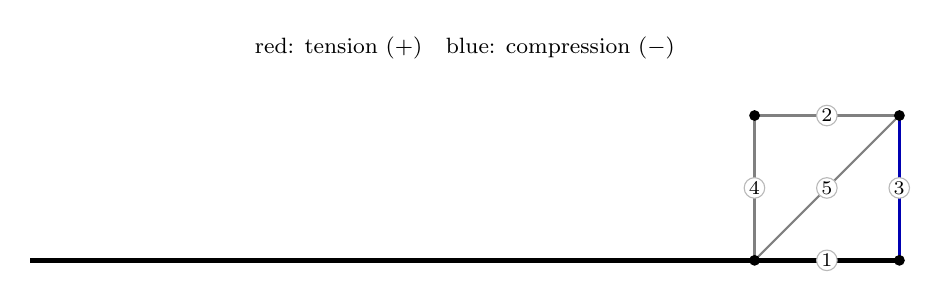
\begin{tikzpicture}[scale=1.226,>=Stealth,line join=round]
  \coordinate (P0) at (0.000,0.000);
  \coordinate (G) at (3.000,0.000);
  \coordinate (D) at (6.000,0.000);
  \coordinate (P1) at (9.000,0.000);
  \coordinate (TO1) at (7.500,0.000);
  \coordinate (TU0) at (9.000,1.500);
  \coordinate (TU1) at (7.500,1.500);
  \draw[thick,gray] (P1) -- (TO1);
  \draw[thick,gray] (TU0) -- (TU1);
  \draw[thick,blue!70!black] (P1) -- (TU0);
  \draw[thick,gray] (TO1) -- (TU1);
  \draw[thick,gray] (TU0) -- (TO1);
  \draw[line width=2pt] (P0) -- (G);
  \draw[line width=2pt] (G) -- (D);
  \draw[line width=2pt] (D) -- (P1);
  \fill (P1) circle (1.6pt);
  \fill (TO1) circle (1.6pt);
  \fill (TU0) circle (1.6pt);
  \fill (TU1) circle (1.6pt);
  \node[circle,fill=white,draw=gray!55,inner sep=0.5pt,font=\scriptsize] at (8.250,0.000) {1};
  \node[circle,fill=white,draw=gray!55,inner sep=0.5pt,font=\scriptsize] at (8.250,1.500) {2};
  \node[circle,fill=white,draw=gray!55,inner sep=0.5pt,font=\scriptsize] at (9.000,0.750) {3};
  \node[circle,fill=white,draw=gray!55,inner sep=0.5pt,font=\scriptsize] at (7.500,0.750) {4};
  \node[circle,fill=white,draw=gray!55,inner sep=0.5pt,font=\scriptsize] at (8.250,0.750) {5};
  \node[font=\footnotesize] at (4.50,2.20) {red: tension $(+)$\quad blue: compression $(-)$};
\end{tikzpicture}
\end{center}
\par\medskip\textbf{4.\ Section-force diagrams of the beams}\par
\begin{center}
\textbf{Beam 1}\\[2pt]
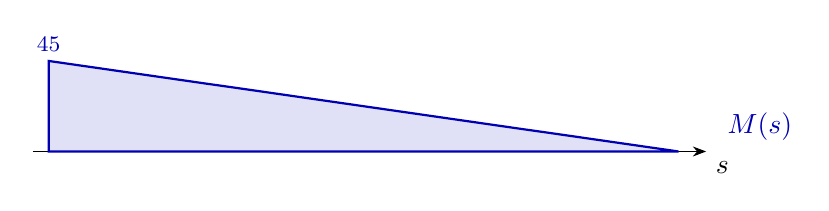
\begin{tikzpicture}[>=Stealth]
  \draw[->] (-0.2,0) -- (8.35,0) node[below right]{$s$};
  \filldraw[fill=blue!70!black!12,draw=blue!70!black,thick] (0,0) -- plot coordinates {(0.000,1.150) (0.333,1.102) (0.667,1.054) (1.000,1.006) (1.333,0.958) (1.667,0.910) (2.000,0.862) (2.333,0.815) (2.667,0.767) (3.000,0.719) (3.333,0.671) (3.667,0.623) (4.000,0.575) (4.333,0.527) (4.667,0.479) (5.000,0.431) (5.333,0.383) (5.667,0.335) (6.000,0.287) (6.333,0.240) (6.667,0.192) (7.000,0.144) (7.333,0.096) (7.667,0.048) (8.000,0.000)} -- (8.000,0) -- cycle;
  \node[above,blue!70!black,font=\footnotesize] at (0.000,1.150) {45};
  \node[blue!70!black,right] at (8.50,0.32) {$M(s)$};
\end{tikzpicture}\\[5pt]
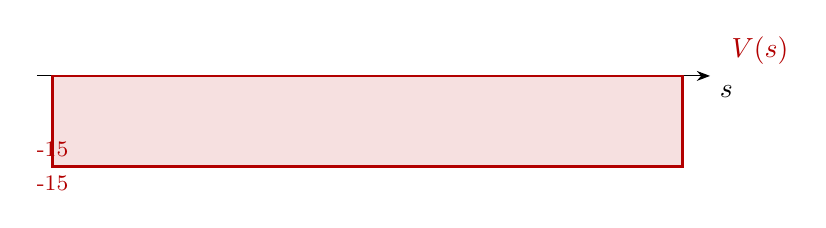
\begin{tikzpicture}[>=Stealth]
  \draw[->] (-0.2,0) -- (8.35,0) node[below right]{$s$};
  \filldraw[fill=red!70!black!12,draw=red!70!black,thick] (0,0) -- plot coordinates {(0.000,-1.150) (0.333,-1.150) (0.667,-1.150) (1.000,-1.150) (1.333,-1.150) (1.667,-1.150) (2.000,-1.150) (2.333,-1.150) (2.667,-1.150) (3.000,-1.150) (3.333,-1.150) (3.667,-1.150) (4.000,-1.150) (4.333,-1.150) (4.667,-1.150) (5.000,-1.150) (5.333,-1.150) (5.667,-1.150) (6.000,-1.150) (6.333,-1.150) (6.667,-1.150) (7.000,-1.150) (7.333,-1.150) (7.667,-1.150) (8.000,-1.150)} -- (8.000,0) -- cycle;
  \node[above,red!70!black,font=\footnotesize] at (0.000,-1.150) {-15};
  \node[below,red!70!black,font=\footnotesize] at (0.000,-1.150) {-15};
  \node[red!70!black,right] at (8.50,0.32) {$V(s)$};
\end{tikzpicture}\\[5pt]
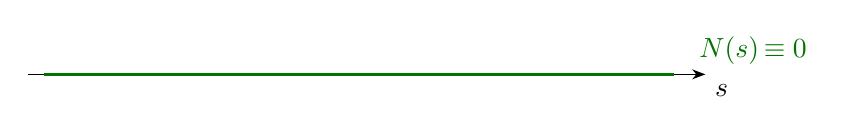
\begin{tikzpicture}[>=Stealth]
  \draw[->] (-0.2,0) -- (8.40,0) node[below right]{$s$};
  \draw[green!45!black,very thick] (0,0) -- (8,0);
  \node[green!45!black,right] at (8.2,0.3) {$N(s)$\,$\equiv 0$};
\end{tikzpicture}\\[10pt]
\textbf{Beam 2}\\[2pt]
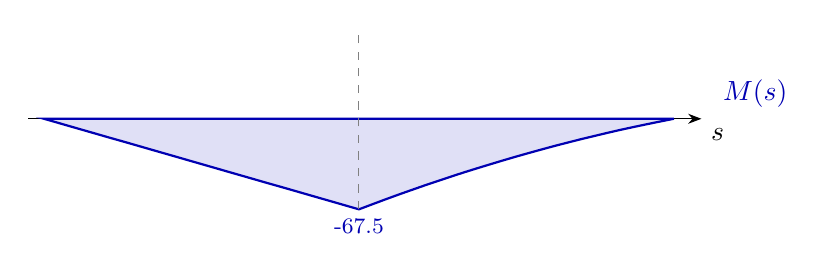
\begin{tikzpicture}[>=Stealth]
  \draw[->] (-0.2,0) -- (8.35,0) node[below right]{$s$};
  \filldraw[fill=blue!70!black!12,draw=blue!70!black,thick] (0,0) -- plot coordinates {(0.000,0.000) (0.167,-0.048) (0.333,-0.096) (0.500,-0.144) (0.667,-0.192) (0.833,-0.240) (1.000,-0.287) (1.167,-0.335) (1.333,-0.383) (1.500,-0.431) (1.667,-0.479) (1.833,-0.527) (2.000,-0.575) (2.167,-0.623) (2.333,-0.671) (2.500,-0.719) (2.667,-0.767) (2.833,-0.815) (3.000,-0.862) (3.167,-0.910) (3.333,-0.958) (3.500,-1.006) (3.667,-1.054) (3.833,-1.102) (4.000,-1.150) (4.000,-1.150) (4.167,-1.087) (4.333,-1.025) (4.500,-0.964) (4.667,-0.905) (4.833,-0.847) (5.000,-0.791) (5.167,-0.735) (5.333,-0.681) (5.500,-0.629) (5.667,-0.578) (5.833,-0.528) (6.000,-0.479) (6.167,-0.432) (6.333,-0.386) (6.500,-0.341) (6.667,-0.298) (6.833,-0.256) (7.000,-0.216) (7.167,-0.176) (7.333,-0.138) (7.500,-0.102) (7.667,-0.067) (7.833,-0.033) (8.000,0.000)} -- (8.000,0) -- cycle;
  \draw[gray,dashed,thin] (4.000,-1.15) -- (4.000,1.15);
  \node[below,blue!70!black,font=\footnotesize] at (4.000,-1.150) {-67.5};
  \node[blue!70!black,right] at (8.50,0.32) {$M(s)$};
\end{tikzpicture}\\[5pt]
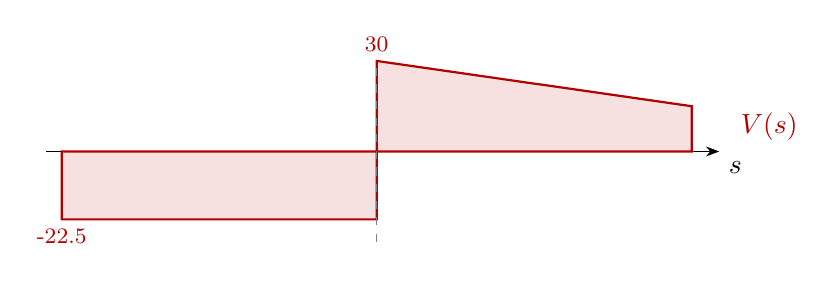
\begin{tikzpicture}[>=Stealth]
  \draw[->] (-0.2,0) -- (8.35,0) node[below right]{$s$};
  \filldraw[fill=red!70!black!12,draw=red!70!black,thick] (0,0) -- plot coordinates {(0.000,-0.862) (0.167,-0.862) (0.333,-0.862) (0.500,-0.862) (0.667,-0.862) (0.833,-0.862) (1.000,-0.862) (1.167,-0.862) (1.333,-0.862) (1.500,-0.862) (1.667,-0.862) (1.833,-0.862) (2.000,-0.862) (2.167,-0.862) (2.333,-0.862) (2.500,-0.862) (2.667,-0.862) (2.833,-0.862) (3.000,-0.862) (3.167,-0.862) (3.333,-0.862) (3.500,-0.862) (3.667,-0.862) (3.833,-0.862) (4.000,-0.862) (4.000,1.150) (4.167,1.126) (4.333,1.102) (4.500,1.078) (4.667,1.054) (4.833,1.030) (5.000,1.006) (5.167,0.982) (5.333,0.958) (5.500,0.934) (5.667,0.910) (5.833,0.886) (6.000,0.862) (6.167,0.839) (6.333,0.815) (6.500,0.791) (6.667,0.767) (6.833,0.743) (7.000,0.719) (7.167,0.695) (7.333,0.671) (7.500,0.647) (7.667,0.623) (7.833,0.599) (8.000,0.575)} -- (8.000,0) -- cycle;
  \draw[gray,dashed,thin] (4.000,-1.15) -- (4.000,1.15);
  \node[above,red!70!black,font=\footnotesize] at (4.000,1.150) {30};
  \node[below,red!70!black,font=\footnotesize] at (0.000,-0.862) {-22.5};
  \node[red!70!black,right] at (8.50,0.32) {$V(s)$};
\end{tikzpicture}\\[5pt]
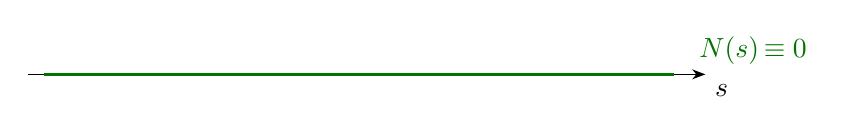
\begin{tikzpicture}[>=Stealth]
  \draw[->] (-0.2,0) -- (8.40,0) node[below right]{$s$};
  \draw[green!45!black,very thick] (0,0) -- (8,0);
  \node[green!45!black,right] at (8.2,0.3) {$N(s)$\,$\equiv 0$};
\end{tikzpicture}\\[10pt]
\end{center}
\end{document}